\documentclass[./PianoDiProgetto.tex]{subfiles}
\begin{document}
\newpage
	\section{Preventivo}
		\subsection{Dettaglio fasi}
			\subsubsection{\PerAR}
				\paragraph{Suddivisione del lavoro}\
	\begin{table}[H]
		%\centering
		\begin{tabularx}{\textwidth}{l*{6}{c}c}
			\toprule
			\textbf{Nominativo} & \textbf{Rp} & \textbf{Am} & \textbf{Pt} 
						& \textbf{An} & \textbf{Pm} & \textbf{Ve} & \textbf{Ore totali} \\
			\midrule
			Andrea Magnan & 0 & 10 &	0 &	8 & 0 & 7 & 28 \\
			%\midrule
			Luca Bertolini & 3 & 7 & 0 & 0 & 0 & 17 & 27 \\
			%\midrule
			Mattia Bottaro &	0 &	10 & 0 & 7 & 0 & 10 & 27 \\
			%\midrule
			Mauro Carlin & 0 & 13 &	0 &	10 & 0 & 3 & 26 \\
			%\midrule
			Nicola Tintorri &	0 & 10 & 0 & 7 & 0 & 10 & 27 \\
			%\midrule
			Pier Paolo Tricomi & 8 & 3 &	0 &	13 & 0 & 4 & 28 \\
			%\midrule
			Simeone Pizzi & 11 & 4 & 0 & 14 & 0 & 0 & 26 \\
			\midrule			
			\textbf{Ore Totali Ruolo} & 22 & 57 & 0 & 59 &	0 &	51 & 189 \\
			\bottomrule
		\end{tabularx}
		\caption{\PerAR{} - Suddivisione delle ore di lavoro}
		%\label{tab:faseA_ore}
	\end{table}
	
	\vspace{15 mm}	
	
	\begin{figure}[H]
		\centering
		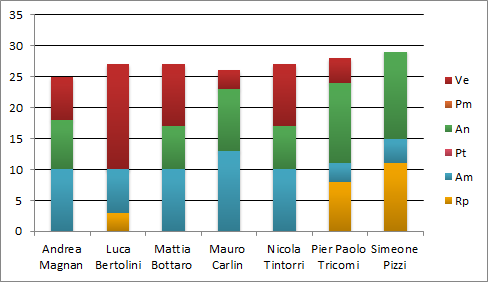
\includegraphics[width=11cm, trim=1cm 0cm 1cm 0cm]{grafici/Ar-persona}
			\caption{\PerAR{} - Riassunto}
		%\label{fig:BarChart-faseA_ore}
	\end{figure}	
	
\newpage
	\vfill	
	\paragraph{Prospetto economico}\
	
	\begin{table}[H]
		\centering
		\begin{tabular}{l * {2}{c}}
			\toprule
			\textbf{Ruolo} & \textbf{Ore} & \textbf{Costo(\euro{})} \\
			\midrule
			Responsabile &	22 &  660,00 \\
			%\midrule
			Amministratore & 57 &  1.140,00 \\
			%\midrule
			Progettista & 0 & 0,00 \\
			%\midrule
			Analista & 59 & 1.475,00 \\
			%\midrule
			Programmatore & 0 & 0,00 \\
			%\midrule
			Verificatore & 51 & 765,00 \\
			\midrule		
			\textbf{Totale} & 189 & 4.040,00 \\
			\bottomrule	
		\end{tabular}
		\caption{\PerAR{} - Costo per ruolo}
		%\label{tab:faseA_costo}
	\end{table}

\vspace{35 mm}	

	\begin{figure}[H]
		\centering
		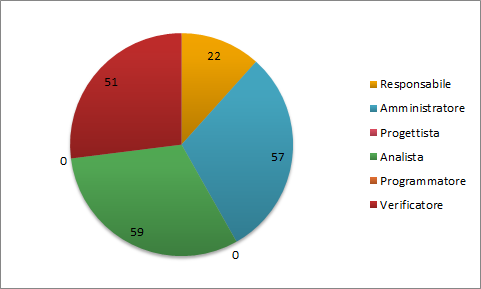
\includegraphics[width=11cm, trim=1cm 0cm 1cm 0cm]{grafici/AR-ruolo}
			\caption{\PerAR{} - Ore per ruolo}
		%\label{fig:CircleChart-faseA_ore_r}
	\end{figure}
	\vfill
	\newpage
	\vfill	
	\begin{figure}[H]
		\centering
		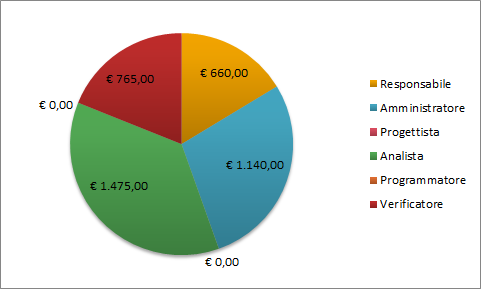
\includegraphics[width=11cm, trim=1cm 0cm 1cm 0cm]{grafici/AR-costo}
			\caption{\PerAR{} - Costo per ruolo}
		%\label{fig:CircleChart-faseA_costo}
	\end{figure}

\vspace{20 mm}
	
	\subsubsection{\PerAD}
				\paragraph{Suddivisione del lavoro}\
				
	\begin{table}[H]
		%\centering
		\begin{tabularx}{\textwidth}{l  * {6}{c}  c}
			\toprule
			\textbf{Nominativo} & \textbf{Rp} & \textbf{Am} & \textbf{Pt} 
						& \textbf{An} & \textbf{Pm} & \textbf{Ve} & \textbf{Ore totali} \\
			\midrule
			Andrea Magnan & 0 & 8 &	0 &	0 & 0 & 4 & 12 \\
			%\midrule
			Luca Bertolini & 0 & 8 & 0 & 0 & 0 & 4 & 12 \\
			%\midrule
			Mattia Bottaro & 0 & 0 & 0 & 8 & 0 & 4 & 12 \\
			%\midrule
			Mauro Carlin & 0 & 0 &	0 &	8 & 0 & 4 & 12 \\
			%\midrule
			Nicola Tintorri &	6 & 6 & 0 & 0 & 0 & 0 & 12 \\
			%\midrule
			Pier Paolo Tricomi & 0 & 0 &	0 &	7 & 0 & 5 & 12 \\
			%\midrule
			Simeone Pizzi & 0 & 0 & 0 & 7 & 0 & 5 & 12 \\
			\midrule			
			\textbf{Ore Totali Ruolo} & 6 & 22 & 0 & 30 & 0 & 26 & 84 \\
			\bottomrule
		\end{tabularx}	
		\caption{\PerAD{} - Suddivisione delle ore di lavoro}
		%\label{tab:faseAD_ore}	
	\end{table}
\newpage

	\vspace{15 mm}	
	
	
	\begin{figure}[H]
		\centering
		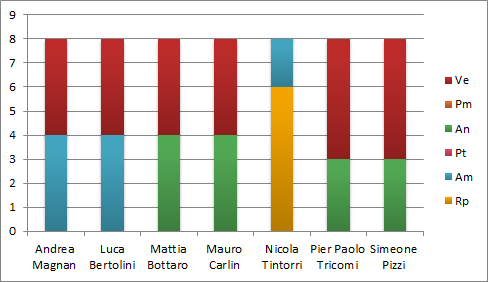
\includegraphics[width=11cm, trim=1cm 0cm 1cm 0cm]{grafici/Ad-persona}
			\caption{\PerAD{} - Riassunto}
		%\label{fig:BarChart-faseAD_ore}
	\end{figure}
	
\vspace{35 mm}	
	
	\paragraph{Prospetto economico}\
	
					\begin{table}[H]
		\centering
	
		\begin{tabular}{l * {2}{c}}
			\toprule
			\textbf{Ruolo} & \textbf{Ore} & \textbf{Costo (\euro{})} \\
			\midrule
			Responsabile &	6 & 180,00 \\
			%\midrule
			Amministratore & 22 & 440,00 \\
			%\midrule
			Progettista & 0 & 0,00 \\
			%\midrule
			Analista & 30 & 750,00 \\
			%\midrule
			Programmatore & 0 & 0,00 \\
			%\midrule
			Verificatore & 26 & 390,00 \\
			\midrule		
			\textbf{Totale} & 84 & 1.760,00 \\
			\bottomrule 
		\end{tabular}
		\caption{\PerAD{} - Costo per ruolo}
		%\label{tab:faseAD_costo}
	\end{table}
\vfill
\newpage
	
	\begin{figure}[H]
		\centering
		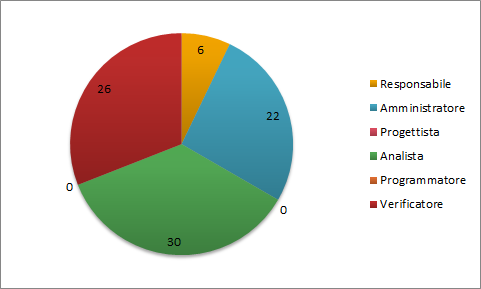
\includegraphics[width=11cm, trim=1cm 0cm 1cm 0cm]{grafici/Ad-ruolo}
			\caption{\PerAD{} - Ore per ruolo}
		%\label{fig:CircleChart-faseAD_ore_r}
	\end{figure}
\vfill
	\begin{figure}[H]
		\centering
		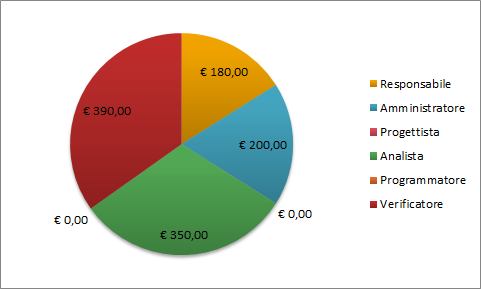
\includegraphics[width=11cm, trim=1cm 0cm 1cm 0cm]{grafici/Ad-costo}
			\caption{\PerAD{} - Costo per ruolo}
		%\label{fig:CircleChart-faseAD_costo}
	\end{figure}
\vfill		
\newpage	
	\subsubsection{\PerPA}
				\paragraph{Suddivisione del lavoro}\
						
	\begin{table}[H]
		\centering
	
		\begin{tabularx}{\textwidth}{l  * {6}{c}  c}
			\toprule
			\textbf{Nominativo} & \textbf{Rp} & \textbf{Am} & \textbf{Pt} 
						& \textbf{An} & \textbf{Pm} & \textbf{Ve} & \textbf{Ore totali} \\
			\midrule
			Andrea Magnan  & 0 & 0 & 0 & 18 & 0 & 8 & 26 \\
			Luca Bertolini  & 0 & 6 & 0 & 12 & 0 & 8 & 26 \\
			Mattia Bottaro  & 7 & 0 & 3 & 9 & 0 & 7 & 26 \\
			Mauro Carlin  & 0 & 0 & 10 & 7 & 0 & 9 & 26 \\
			Nicola Tintorri  & 0 & 0 & 13 & 8 & 0 & 4 & 25 \\
			Pier Paolo Tricomi  & 0 & 10 & 6 & 0 & 0 & 9 & 25 \\
			Simeone Pizzi & 0 & 12 & 8 & 0 & 0 & 5 & 25 \\
			\midrule
			\textbf{Ore Totali Ruolo} & 7 & 28 & 40 & 54 & 0 & 50 & 179 \\
			\bottomrule
		\end{tabularx}
		\caption{\PerPA{} - Suddivisione delle ore di lavoro}
		%\label{tab:fasePA_ore}
	\end{table}
\vfill	
	
	\begin{figure}[H]
		\centering
		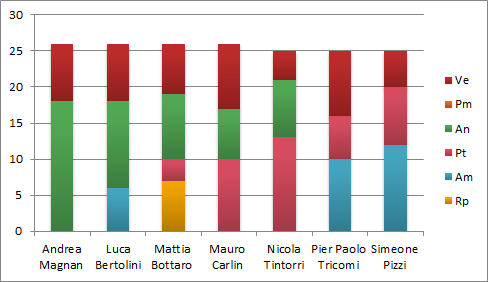
\includegraphics[width=11cm, trim=1cm 0cm 1cm 0cm]{grafici/Pa-persona}
			\caption{\PerPA{} - Riassunto}
		%\label{fig:BarChart-fasePA_ore}
	\end{figure}
\vfill	
\newpage
	
	\paragraph{Prospetto economico}\
					
	\begin{table}[H]
		\centering
	
		\begin{tabular}{l * {2}{c}}
			\toprule
			\textbf{Ruolo} & \textbf{Ore} & \textbf{Costo (\euro{})} \\
			\midrule
			Responsabile & 7    & 210,00 \\
			Amministratore  & 28    & 560,00 \\
			Progettista  & 40    & 880,00 \\
			Analista & 54    & 1.350,00 \\
			Programmatore  & 0    & 0,00 \\
			Verificatore  & 50    & 750,00 \\
			\midrule
			\textbf{Totale}  & 179   & 3.750,00 \\
			\bottomrule
		\end{tabular}
		\caption{\PerPA{} - Costo per ruolo}
		%\label{tab:fasePA_costo}
	\end{table}
\vfill	
	
	\begin{figure}[H]
		\centering
		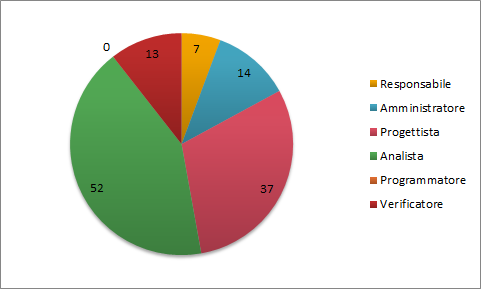
\includegraphics[width=11cm, trim=1cm 0cm 1cm 0cm]{grafici/Pa-ruolo}
			\caption{\PerPA{} - Ore per ruolo}
		%\label{fig:CircleChart-fasePA_ore_r}
	\end{figure}
\vfill	
\newpage
\vfill
	\begin{figure}[H]
		\centering
		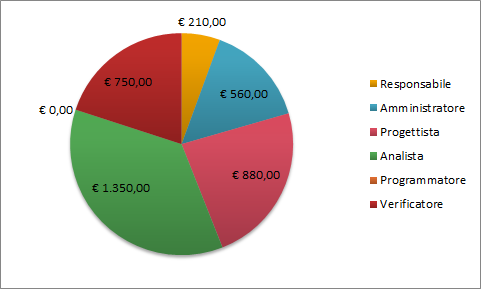
\includegraphics[width=11cm, trim=1cm 0cm 1cm 0cm]{grafici/Pa-costo}
			\caption{\PerPA{} - Costo per ruolo}
		%\label{fig:CircleChart-fasePA_costo}
	\end{figure}	
\vfill	
	\subsubsection{\PerPD}
				\paragraph{Suddivisione del lavoro}\
					
	
	\begin{table}[H]
		%\centering
	
		\begin{tabularx}{\textwidth}{l  * {6}{c}  c}
			\toprule
			\textbf{Nominativo} & \textbf{Rp} & \textbf{Am} & \textbf{Pt} 
						& \textbf{An} & \textbf{Pm} & \textbf{Ve} & \textbf{Ore totali} \\
			\midrule
			Andrea Magnan  & 3 & 4 & 11 & 0 & 0 & 6 & 24 \\
			Luca Bertolini  & 6 & 0 & 6 & 2 & 0 & 10 & 24 \\
			Mattia Bottaro  & 0 & 0 & 6 & 5 & 0 & 13 & 24 \\
			Mauro Carlin  & 0 & 13 & 0 & 4 & 0 & 7 & 24 \\
			Nicola Tintorri  & 0 & 2 & 0 & 14 & 0 & 8 & 24 \\
			Pier Paolo Tricomi  & 0 & 0 & 9 & 10 & 0 & 5 & 24 \\
			Simeone Pizzi & 0 & 0 & 8 & 8 & 0 & 8 & 24 \\
			\midrule			
			\textbf{Ore Totali Ruolo}& 9 & 19 & 40 & 43 & 0 & 57 & 168 \\
			\bottomrule	
		\end{tabularx}
		\caption{\PerPD{} - Suddivisione delle ore di lavoro}
		
	\end{table}
\vfill
\newpage
\vfill	
		
	\begin{figure}[H]
		\centering
		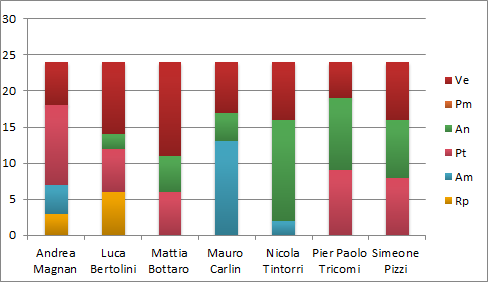
\includegraphics[width=11cm, trim=1cm 0cm 1cm 0cm]{grafici/Pd-persona}
			\caption{\PerPD{} - Riassunto}
		
	\end{figure}
\vfill	
	\paragraph{Prospetto economico}\
					
	\begin{table}[H]
		\centering
	
		\begin{tabular}{l * {2}{c}}
			\toprule
			\textbf{Ruolo} & \textbf{Ore} & \textbf{Costo (\euro{})} \\
			\midrule
			Responsabile & 9    &  270,00 \\
			Amministratore  & 19     &  380,00 \\
			Progettista  & 40    &  880,00 \\
			Analista & 43   &  1.075,00 \\
			Programmatore  & 0    &  0,00 \\
			Verificatore  & 57    &  855,00 \\
			\midrule
			\textbf{Totale}  & 168   &  3.460,00 \\
			\bottomrule		
		\end{tabular}
		\caption{\PerPD{} - Costo per ruolo}
		
	\end{table}
\vfill	
\newpage
\vfill
	
	\begin{figure}[H]
		\centering
		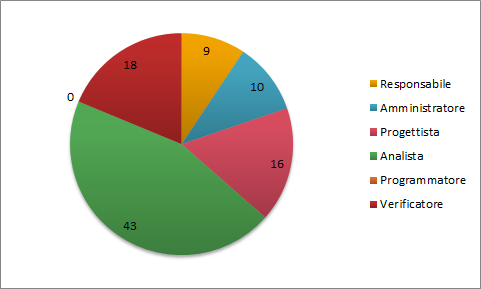
\includegraphics[width=11cm, trim=1cm 0cm 1cm 0cm]{grafici/Pd-ruolo}
			\caption{\PerPD{}- Ore per ruolo}
		
	\end{figure}

\vfill	
	\begin{figure}[H]
		\centering
		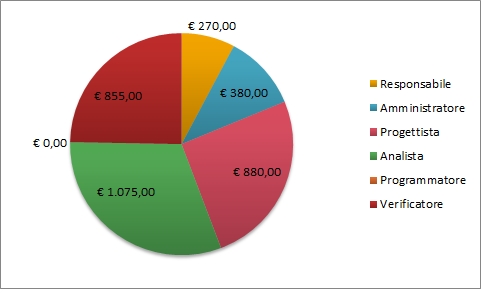
\includegraphics[width=11cm, trim=1cm 0cm 1cm 0cm]{grafici/Pd-costo}
			\caption{\PerPD{} - Costo per ruolo}
	\end{figure}
\vfill	
\newpage	
	
	\subsubsection{\PerC}
				\paragraph{Suddivisione del lavoro}\
						
	\begin{table}[H]
		%\centering
		\begin{tabularx}{\textwidth}{l  * {6}{c}  c}
			\toprule
			\textbf{Nominativo} & \textbf{Rp} & \textbf{Am} & \textbf{Pt} 
						& \textbf{An} & \textbf{Pm} & \textbf{Ve} & \textbf{Ore totali} \\
			\midrule
			Andrea Magnan  & 3 & 0 & 11 & 0 & 5 & 11 & 30 \\
			Luca Bertolini  & 0 & 7 & 12 & 0 & 12 & 0 & 31 \\
			Mattia Bottaro  & 0 & 10 & 10 & 0 & 11 & 0 & 31 \\
			Mauro Carlin  & 7 & 0 & 9 & 0 & 12 & 3 & 31 \\
			Nicola Tintorri  & 0 & 0 & 0 & 0 & 16 & 17 & 33 \\
			Pier Paolo Tricomi  & 0 & 0 & 8 & 0 & 16 & 7 & 31 \\
			Simeone Pizzi & 4 & 0 & 4 & 0 & 19 & 4 & 31 \\
			\midrule
			\textbf{Ore Totali Ruolo} & 14 & 17 & 54 & 0 & 91 & 42 & 218 \\
			\bottomrule
			
		\end{tabularx}
		\caption{\PerC{} - Suddivisione delle ore di lavoro}
	\end{table}
	
\vfill	
		
	\begin{figure}[H]
		\centering
		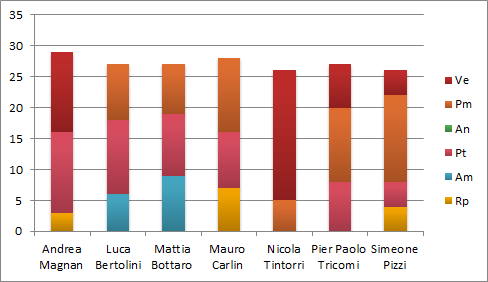
\includegraphics[width=11cm, trim=1cm 0cm 1cm 0cm]{grafici/C-persona}
			\caption{\PerC{}- Riassunto}
	\end{figure}
\vfill	
	
	\paragraph{Prospetto economico}\
					
	\begin{table}[H]
		\centering
	
		\begin{tabular}{l * {2}{c}}
			\toprule
			\textbf{Ruolo} & \textbf{Ore} & \textbf{Costo (\euro{})} \\
			\midrule
			Responsabile & 14    &  420,00 \\
			Amministratore  & 17    &  340,00 \\
			Progettista  & 54   &  1.188,00 \\
			Analista & 0    &  0,00 \\
			Programmatore  & 91    &  1.365,00 \\
			Verificatore  & 42    &  630,00 \\
			\midrule
			\textbf{Totale}  & 218   &  3.943,00 \\
			\bottomrule
		\end{tabular}
		\caption{\PerC{} - Costo per ruolo}
	\end{table}

\vspace{35mm}
	
	\begin{figure}[H]
		\centering
		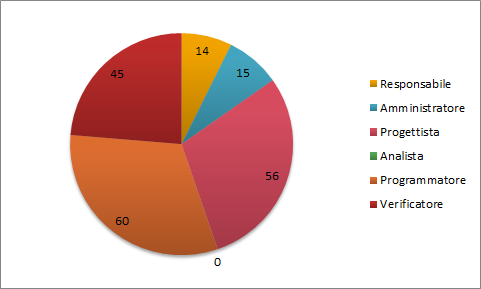
\includegraphics[width=11cm, trim=1cm 0cm 1cm 0cm]{grafici/C-ruolo}
			\caption{\PerC{} - Ore per ruolo}
	\end{figure}
\vfill
	\begin{figure}[H]
		\centering
		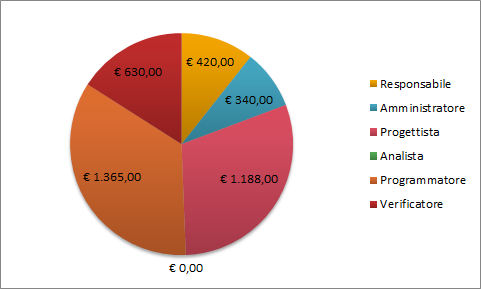
\includegraphics[width=11cm, trim=1cm 0cm 1cm 0cm]{grafici/C-costo}
			\caption{\PerC{} - Costo per ruolo}
	\end{figure}
	
\vspace{35mm}	
	
	
	\subsubsection{\PerV}
				\paragraph{Suddivisione del lavoro}\
					
	\begin{table}[H]
		%\centering
		\begin{tabularx}{\textwidth}{l  * {6}{c}  c}
			\toprule
			\textbf{Nominativo} & \textbf{Rp} & \textbf{Am} & \textbf{Pt} 
						& \textbf{An} & \textbf{Pm} & \textbf{Ve} & \textbf{Ore totali} \\
			\midrule
			Andrea Magnan  & 0 & 0 & 0 & 0 & 6 & 7 & 13 \\
			Luca Bertolini  & 0 & 0 & 0 & 0 & 8 & 4 & 12 \\
			Mattia Bottaro  & 0 & 0 & 5 & 0 & 0 & 7 & 12 \\
			Mauro Carlin  & 0 & 8 & 0 & 0 & 0 & 4 & 12 \\
			Nicola Tintorri  & 0 & 3 & 0 & 0 & 0 & 8 & 11 \\
			Pier Paolo Tricomi  & 7 & 0 & 0 & 0 & 4 & 2 & 13 \\
			Simeone Pizzi & 0 & 0 & 0 & 0 & 2 & 11 & 13 \\
			\midrule
			\textbf{Ore Totali Ruolo} & 7 & 11 & 5 & 0 & 20 & 43 & 86 \\
			\bottomrule
		\end{tabularx}
		\caption{\PerV{} - Suddivisione delle ore di lavoro}
	\end{table}
\vfill	

	
	\begin{figure}[H]
		\centering
		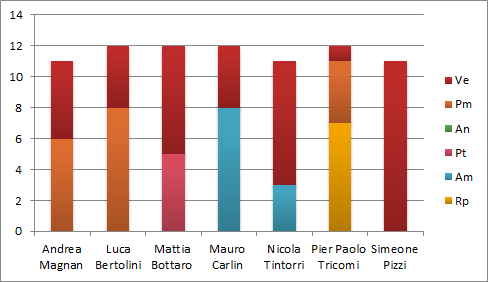
\includegraphics[width=11cm, trim=1cm 0cm 1cm 0cm]{grafici/V-persona}
			\caption{\PerV{} - Riassunto}
	\end{figure}
	
\vspace{35 mm}	
	\paragraph{Prospetto economico}\
					
	\begin{table}[H]
		\centering
	
		\begin{tabular}{l * {2}{c}}
			\toprule
			\textbf{Ruolo} & \textbf{Ore} & \textbf{Costo (\euro{})} \\
			\midrule
			Responsabile & 7 & 210,00 \\
			Amministratore  & 11 & 220,00 \\
			Progettista  & 5 & 110,00 \\
			Analista & 0 & 0,00 \\
			Programmatore  & 20 &  300,00 \\
			Verificatore  & 43 &  645,00 \\
			\midrule
			\textbf{Totale}  & 86   &  1.485,00 \\
			\bottomrule	
		\end{tabular}
		\caption{\PerV{} - Costo per ruolo}
	\end{table}
\vfill	
	
	\begin{figure}[H]
		\centering
		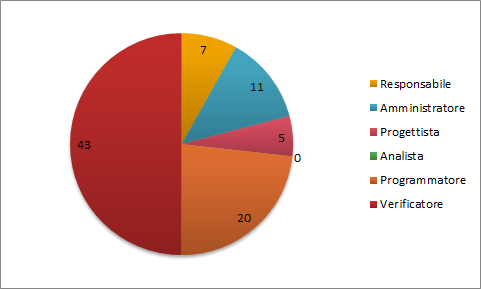
\includegraphics[width=11cm, trim=1cm 0cm 1cm 0cm]{grafici/V-ruolo}
			\caption{\PerV{} - Ore per ruolo}
	\end{figure}
\vfill	

	\begin{figure}[H]
		\centering
		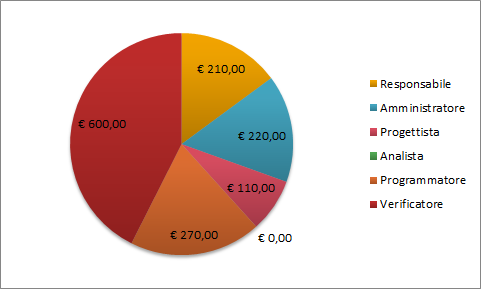
\includegraphics[width=11cm, trim=1cm 0cm 1cm 0cm]{grafici/V-costo}
			\caption{\PerV{} - Costo per ruolo}
	\end{figure}	
	
\vspace{35mm}	
	
	\subsection{Riepilogo}
			\subsubsection{Ore totali rendicontate}
				\paragraph{Suddivisione del lavoro}\
					Le ore totali rendicontate escludono le ore del periodo \PerAR{} in quanto il gruppo \GRUPPO\ non è ancora stato scelto come fornitore ufficiale e sono da considerarsi come ore di investimento. Ogni componente del gruppo \GRUPPO\ dedicherà quindi ad ognuno dei ruoli, a rotazione, le seguenti ore rendicontate:
	
	\begin{table}[H]
		%\centering
		\begin{tabularx}{\textwidth}{l  * {6}{c}  c}
			\toprule
			\textbf{Nominativo} & \textbf{Rp} & \textbf{Am} & \textbf{Pt} 
						& \textbf{An} & \textbf{Pm} & \textbf{Ve} & \textbf{Ore totali} \\
			\midrule
			Andrea Magnan  & 6  & 12 & 22 & 18 & 11  & 36 & 105 \\
			Luca Bertolini  & 6 & 21 & 18 & 14 & 20 & 26 & 105 \\
			Mattia Bottaro  & 7  & 10 & 24 & 22 & 11  & 31 & 105 \\
			Mauro Carlin  & 7 & 21 & 19 & 19 & 12 & 27 & 105 \\
			Nicola Tintorri  & 6 & 11 & 13 & 22 & 17 & 37 & 105 \\
			Pier Paolo Tricomi  & 7 & 10 & 23 & 17 & 20 & 28 & 105 \\
			Simeone Pizzi & 4 & 12 & 20 & 15 & 21 & 33 & 105 \\
			\midrule
			\textbf{Ore Totali Ruolo} & 43    & 97   & 139   & 127   & 111 & 218   & 735 \\
			\bottomrule
		\end{tabularx}
		\caption{Ore totali - Suddivisione delle ore di lavoro}
	\end{table}
	

\vfill
		
	\begin{figure}[H]
		\centering
		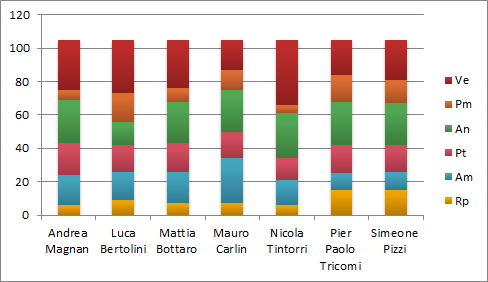
\includegraphics[width=11cm, trim=1cm 0cm 1cm 0cm]{grafici/TOT-persona}
			\caption{Ore persona totali - Riassunto}
		%\label{fig:BarChart-totale_ore}
	\end{figure}
	
\newpage	
	
	\paragraph{Prospetto economico}\
					Il costo totale per ogni ruolo è dunque il seguente:
	\begin{table}[H]
		\centering
		\begin{tabular}{l * {2}{c}}
			\toprule
			\textbf{Ruolo} & \textbf{Ore} & \textbf{Costo (\euro{})} \\
			\midrule
			Responsabile & 43    &  1.290,00 \\
			Amministratore  & 97   &  1.940,00 \\
			Progettista  & 139   &  3.058,00 \\
			Analista & 127   &  3.175,00 \\
			Programmatore  & 111   &  1.665,00 \\
			Verificatore  & 218   &  3.270,00 \\
			\midrule
			\textbf{Totale}  & 735  &  14.398,00 \\
			\bottomrule
			
		\end{tabular}
		\caption{Ore totali - Costo per ruolo}
		%\label{tab:totale_costo}
	\end{table}

\vspace{35 mm}	
	
	\begin{figure}[H]
		\centering
		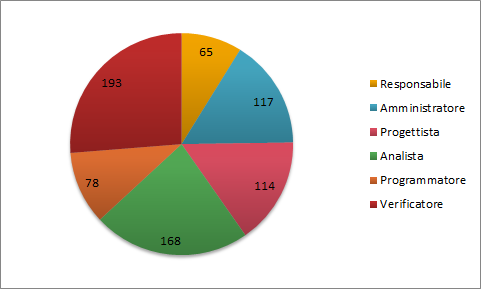
\includegraphics[width=11cm, trim=1cm 0cm 1cm 0cm]{grafici/TOT-ruolo}
			\caption{Ore totali - Ore per ruolo}
		%\label{fig:CircleChart-totale_ore_r}
	\end{figure}	
	
\newpage	
	
\vfill
	\begin{figure}[H]
		\centering
		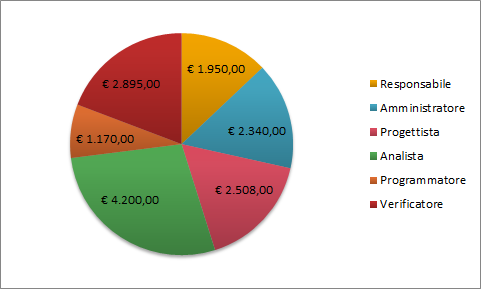
\includegraphics[width=11cm, trim=1cm 0cm 1cm 0cm]{grafici/TOT-costo}
			\caption{Ore totali - Costo per ruolo}
		%\label{fig:CircleChart-totale_ore}
	\end{figure}
\vfill
\newpage		
\end{document}